\section{Problem formulation}
\label{sec:problem-formulation}
In this section, we give an outline of the system model (Subsection~\ref{subsec:system-model}), which is used in the optimisation problem (Subsection~\ref{subsec:optimisation-problem}). We then prove that it is NP-Hard (Subsection~\ref{subsec:time-complexity}) and finally, using an example problem setting (Subsection~\ref{subsec:example-problem-case}), we demonstrate the effectiveness of our flexible resource allocation approach compared to previous work.

\subsection{System model}
\label{subsec:system-model}
We assume that there is a set of servers (i.e., edge nodes) $I = \{1,2,\ldots,\left|I\right|\}$, which can be accessed through either cellular base stations or WiFi access points (APs). These servers have different types of limited resources: storage for the code/data needed to run tasks, computation capacity in terms of CPU cycles per time interval and communication bandwidth to receive data and to send back the results after execution.\footnote{Future work will explore additional attributes like I/O memory access per second, GPU usage, and more.} These servers are also assumed to be heterogeneous in all their characteristics. Formally, we characterise server $i \in I$ with storage capacity $S_i$, computation capacity $W_i$, and bandwidth capacity $R_i$.

There is also a set of computational tasks $J = \{1,2,\ldots, \left| J \right|\}$, that each require service from one of the servers $I$. Each task has a monetary value $v_j$, representing the value of completing the task to its owner. In order to run a task, the server is required to load the task onto the server from a source, to compute it and then send back results to the user. For each of these stages, we consider separate speeds that these operations could occur at.

Formally, task $j \in J$ has storage requirement $s_j$, and we denote the rate that the task is transferred to a server at as $s'_j$. The total number of CPU cycles required for the task to complete is $w_j$, and the number of CPU cycles assigned to the task per time interval is $w'_j$. Finally, the size of the results is denoted as $r_j$, while the bandwidth used to send back results to the user is denoted as $r'_j$.

Furthermore, as tasks in edge computing are typically time-sensitive, each task also has a deadline, denoted by $d_j$, representing the maximum amount of time for a task to be completed successfully within. For tractability, we do not consider the specific timings of retrieving data and sending results. Instead, we take a conservative approach, assuming that they can overlap arbitrarily (as modelled in constraint~\eqref{eq:task-deadline}). Finally, we assume that there is an \emph{all}-or-\emph{nothing} task execution reward, meaning that the task value is derived only if the task is completed within its deadline.

\subsection{Optimisation problem}
\label{subsec:optimisation-problem}
Given the aforementioned assumptions and variables from the system model, an optimisation problem is constructed as follows. The formulation uses the additional variable $x_{i,j} \in \{0,1\}$ to denote whether task $j$ is run on server $i$.

\begin{align}
    \max & \sum_{\forall j \in J} v_j \cdot \left(\sum_{\forall i \in I} x_{i,j}\right) \label{eq:objective} \\
    \mbox{s.t.} \nonumber \\
    & \sum_{\forall j \in J} s_j \cdot x_{i,j} \leq S_i, &~ \forall{i \in I} \label{eq:server-storage-constraint} \\
    & \sum_{\forall j \in J} w'_j \cdot x_{i,j} \leq W_i, &~ \forall{i \in I} \label{eq:server-computation-constraint} \\
    & \sum_{\forall j \in J} (r'_j + s'_j) \cdot x_{i,j} \leq R_i, &~ \forall{i \in I} \label{eq:server-bandwidth-constraint} \\
    & \frac{s_j}{s'_j} + \frac{w_j}{w'_j} + \frac{r_j}{r'_j} \leq d_j, &~ \forall{j \in J} \label{eq:task-deadline} \\
    & 0 < s'_j, &~ \forall{j \in J} \label{eq:loading-speeds} \\
    & 0 < w'_j, &~ \forall{j \in J} \label{eq:compute-speeds} \\
    & 0 < r'_j, &~ \forall{j \in J} \label{eq:sending-speeds} \\
    & \sum_{\forall i \in I} x_{i,j} \leq 1, &~ \forall{j \in J} \label{eq:server-task-allocation} \\
    & x_{i,j} \in \{0, 1\}, &~ \forall{i \in I},\forall{j \in J} \label{eq:task-allocation}
\end{align}

The objective (Eq.\ref{eq:objective}) is to maximise the total value over all tasks (i.e.,\ social welfare) that are completed within their deadline (Eq.~\eqref{eq:task-deadline}). Constraints~(\ref{eq:server-storage-constraint}),~(\ref{eq:server-computation-constraint}) and~(\ref{eq:server-bandwidth-constraint}) each prevent over-allocation of server resources to allocated tasks. To force each task to be completed within its assigned deadline, constraint~(\ref{eq:task-deadline}) requires the sum of time taken for each stage of the task (i.e., sending data, computation and returning results) to be less than the task deadline.\footnote{If a task is not allocated to any server, this constraint can be satisfied by choosing arbitrarily high resource speeds, as this does not use up the resources of any servers.} Finally, constraints~(\ref{eq:server-task-allocation}) and~(\ref{eq:task-allocation}) capture the fact that every task can be served by at most one server.

This model focuses on a single-shot setting, where all tasks arrive at the same time to the system. To use this system in practice, where tasks arrive progressively over time, an allocation mechanism would repeat the allocation decisions over regular time intervals. We leave a more detailed study of online elastic resource allocation mechanisms to future work.

\subsection{Computational complexity}
\label{subsec:time-complexity}
The optimisation problem as described in Subsection~\ref{subsec:optimisation-problem} is an extension of the knapsack problem, a well-studied problem that is known to be NP-hard.

\begin{theorem}
     The optimisation problem (\ref{eq:objective})-(\ref{eq:task-allocation}) is NP-hard.
\end{theorem}
\begin{proof}
% Proof written by fidan
    The optimisation problem without the task deadline constraint (Eq.~(\ref{eq:task-deadline})) is a 0-1 multidimensional knapsack problem~\cite{knapsackproblems_2004}, which is a  generalisations of a simple 0-1 knapsack problems. The latter are NP-hard  problems~\cite{knapsackproblems_2004}. Given this, it follows that the 0-1 multidimensional knapsack problems are also NP-hard. Since optimization problem  (Eqs.~(\ref{eq:objective})-(\ref{eq:task-allocation})) is a generalization of a 0-1 multidimensional knapsack problem, it follows that it is NP-hard as well. 
\end{proof}

\subsection{Example problem case}
\label{subsec:example-problem-case}
Before we propose our mechanisms in the next section, we present an example case to illustrate why considering resource-elastic tasks is important. In this example, there are 3 servers and 12 potential tasks where the flexible resource allocation solution (Figure~\ref{fig:example-flexible-solution}) is able to complete all of the tasks. This is compared to the fixed resource allocation solution (Figure~\ref{fig:example-fixed-solution}) that is only able to achieve 9 tasks. As a result, there is a 21\% difference in social welfare between  the two algorithms. The exact settings can be found in Section 1 of the supplementary material.

\begin{figure}[ht]
    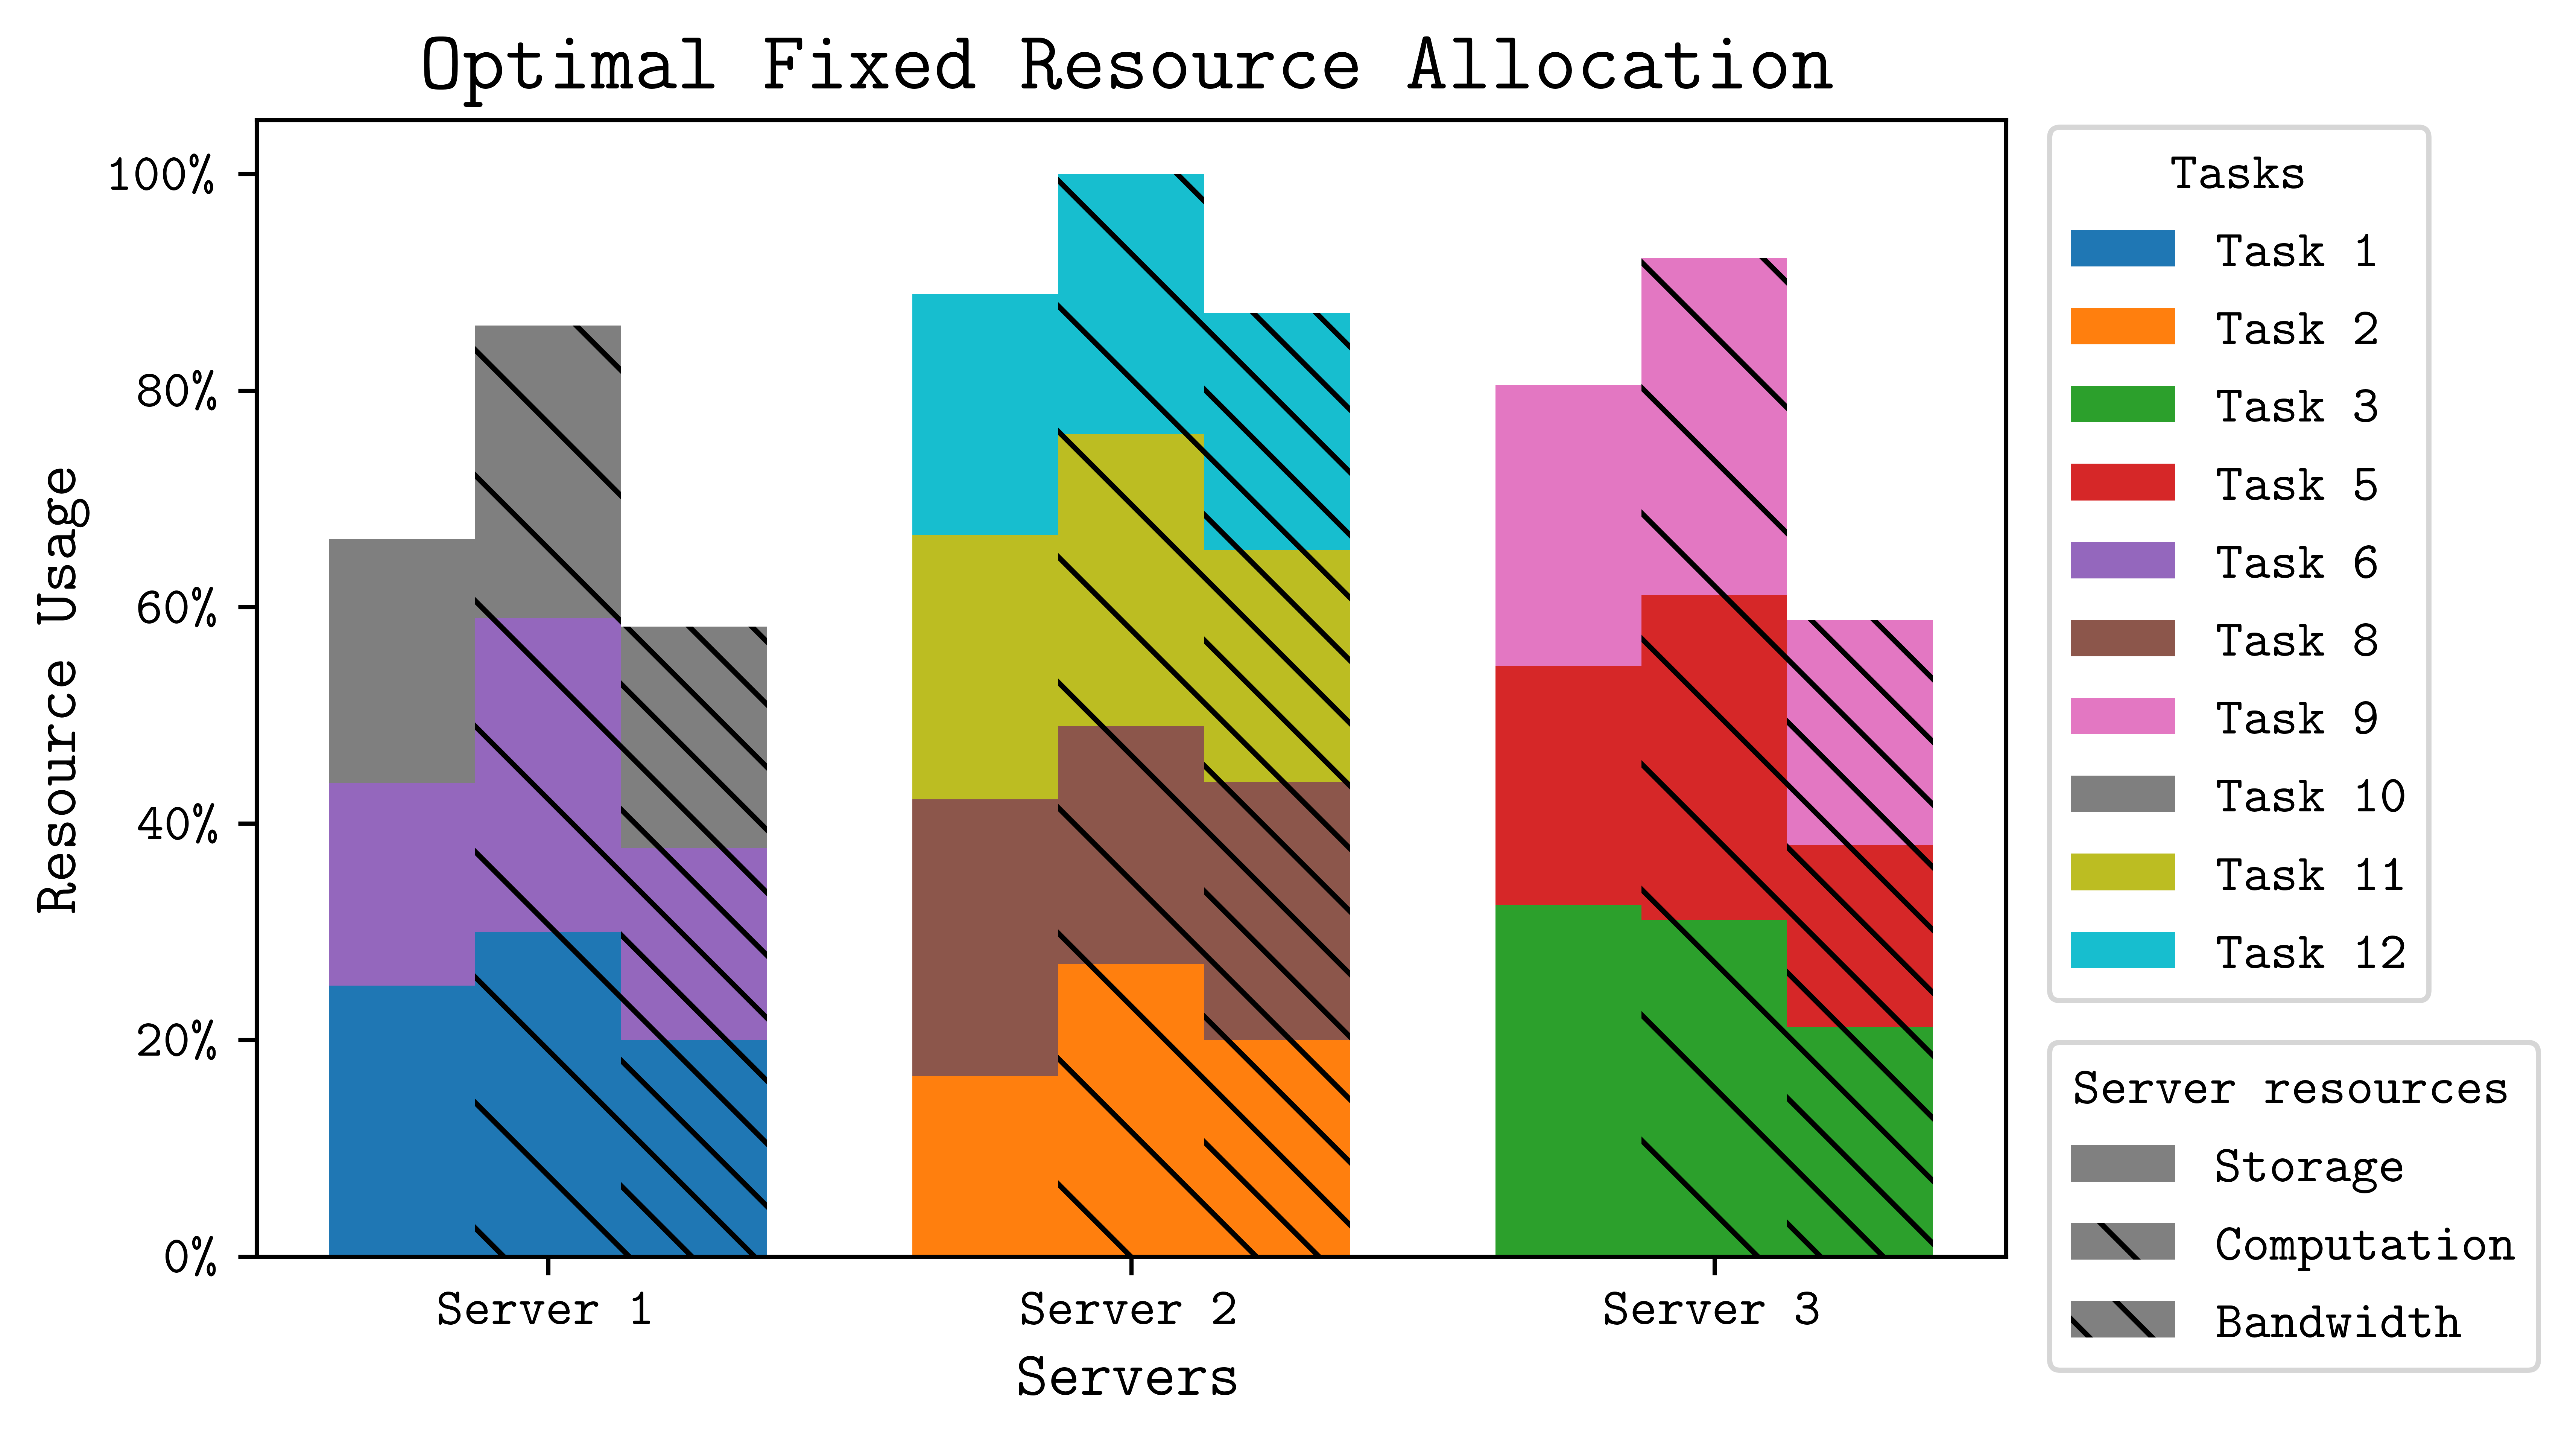
\includegraphics[width=\linewidth]{figs/allocation/optimal_fixed_resource_allocation.png}
    \caption{Optimal solution for example case using fixed resource allocation.}
    \label{fig:example-fixed-solution}
\end{figure}

The figures~\ref{fig:example-fixed-solution} and~\ref{fig:example-flexible-solution} represent each server as a group of three bars, each relating to a server's resource type, with the percentage of resources used by a task being the height of the bar. As server 1 and 3 have limited bandwidth resources, the fixed resource allocation is unable to utilise all of their computational resources compared to the flexible resource allocation, which is able to use almost all of its resources. Due to this ability to utilise more of their resources, the servers are each able to compute 1 more task than the fixed resource allocation.

\begin{figure}[ht]
    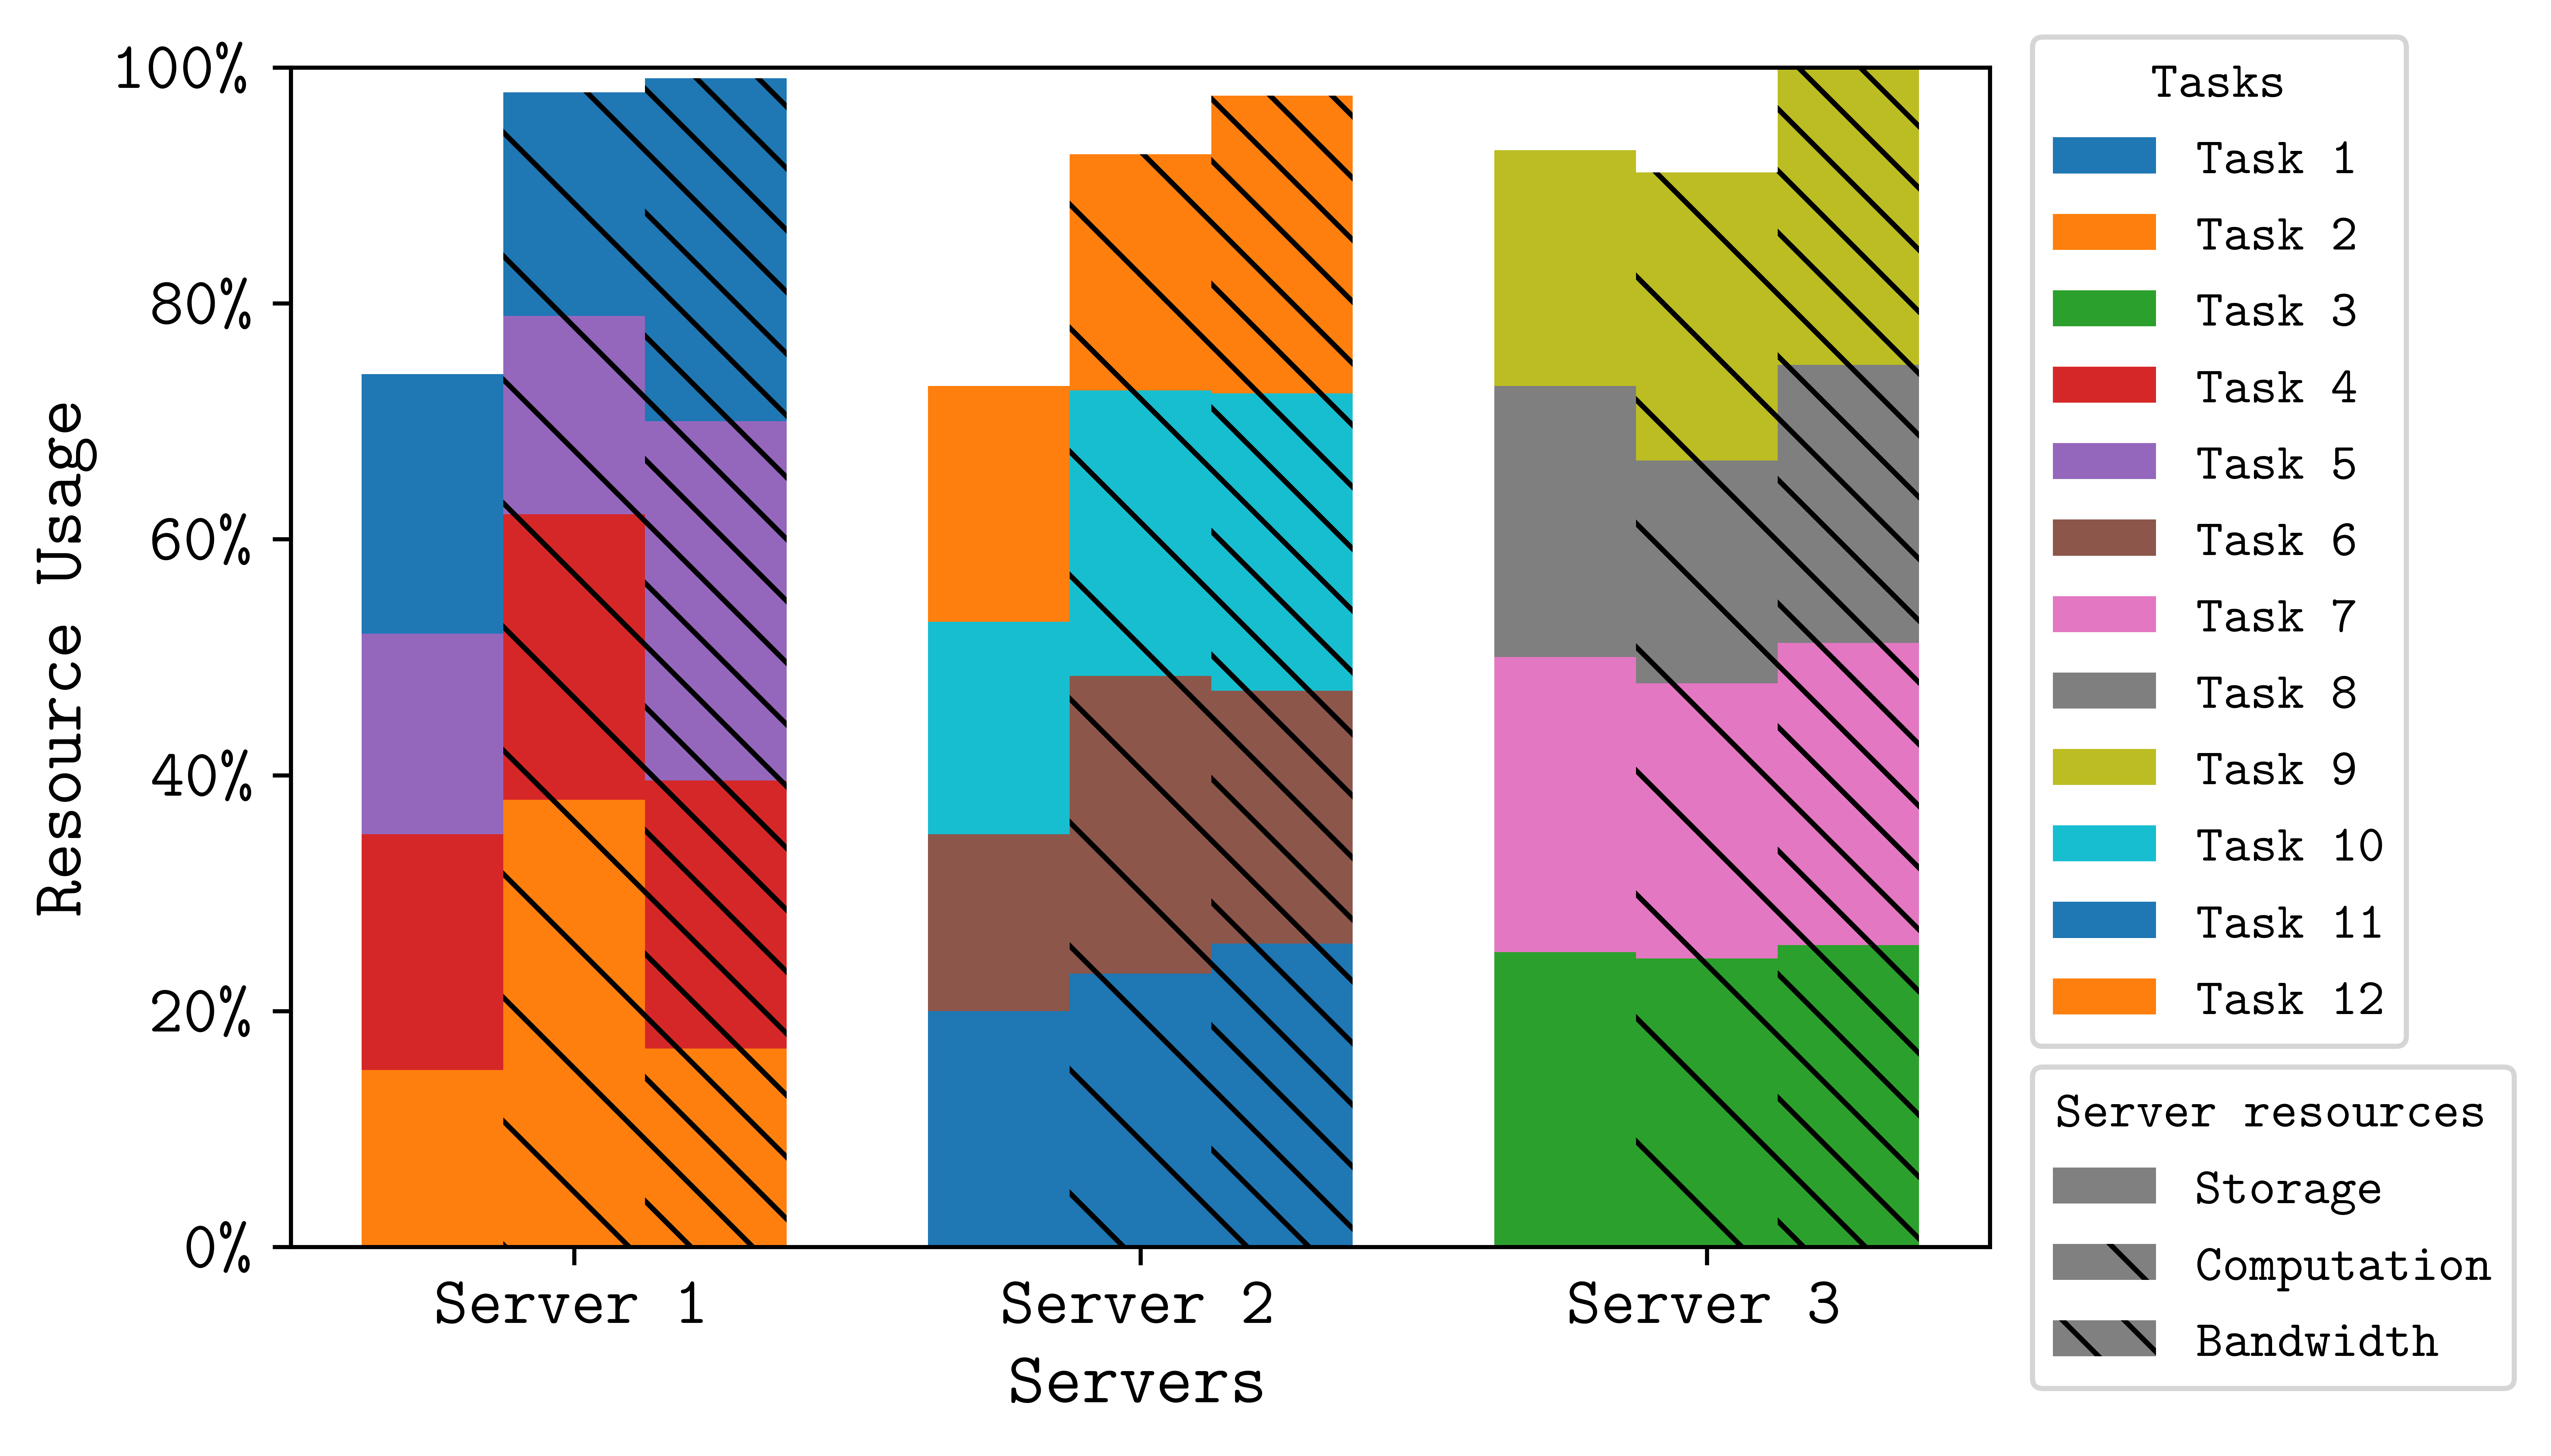
\includegraphics[width=\linewidth]{figs/allocation/optimal_flexible_resource_allocation.png}
    \caption{Optimal solution for example case using our flexible resource allocation.}
    \label{fig:example-flexible-solution}
\end{figure}